\documentclass{article}
\usepackage[utf8]{inputenc}
\usepackage{graphicx}
\graphicspath{ {./images/} }
\usepackage{amsmath}
\usepackage{hyperref}
%\usepackage[english]{babel}

\usepackage[left=2cm,right=1cm, top=2cm,bottom=2cm,bindingoffset=0cm]{geometry}

\renewcommand{\normalsize}{\fontsize{14}{18pt}\selectfont}

\title{Project Assignment}
\author{ Kamilla Faizullina}
\date{\empty}

\begin{document}
\maketitle
 To run programs, we use \href{https://www.nvidia.com/en-us/data-center/v100/}{NVDIA Tesla V100 Nvlink}. Memory bandwidth is  $900$ GB/s and the prformance is $7.8$  teraFLOPS for Double-Precision and $15.7$ teraFLOPS for Single-Precision.

\section{Formats for Sparse Matrix}
A sparse matrix is a matrix that has a lot of zero values. To store such matrix more efficiently than usual two-dimensional matrix, there are special data structures. In this work, we focus only on the Compressed Sparse Row (CSR) format and SELL-C-Sigma approach by Kreutzer (which is extension of ELLPACK structure). 

The implementation of naive CSR (scalar CSR) is 3 arrays: pointers on starts of row (+last element - the number of non-zero elements in matrix), indexes on columns and the values. It is seems not bad that we do not store any extra zeros and data are really compressed (see \ref{formats}). However, the matrix algebra is often used on GPU platform and scalar CSR usually performs not well on GPU.  The problems are memory access pattern. It is supposed that a lot of threads would not process enough non-zeroes values. Scalar CSR could be extended to vectorized CSR for which used  warp per row. According to Kreutzer et al,it is still could be inefficient (However, the performance also depends on the pattern of original matrices). 

The next generalization is ELLPACK which is similar to CSR but includes padding. It is a good approach when the average number of non-zero elements. However, padding is a solve of non coalesced memory accesses of CSR and the other problem at the same time. If one of the rows has too much elements, ELLPACK is inefficient. To overcome this, we can use sliced ELLPACK-S, where for every S rows different number for padding. 

The more general approach is SELL-C-SIGMA. It is sliced ELLPACH-C where every SIGMA elements are sorted. When C=1 and SIGMA=1 it is CRS format. However, low C is not efficient values. According to authors \ref{formats}, this approach is good for GPU as there is no loading of too much extra zeros and each thread run only until the actual row length is reached. However, if number of non-zero element in stored values ($\beta$) it is still could be not so efficient (However, there is no perfect data structure for ). This approach is quite general due to sorting and padding only every C rows. 

Naive ELLPACK is quite easy to implement using Kokkos as there constant number of elements in values. 

 \begin{figure}[h]
	\centering
	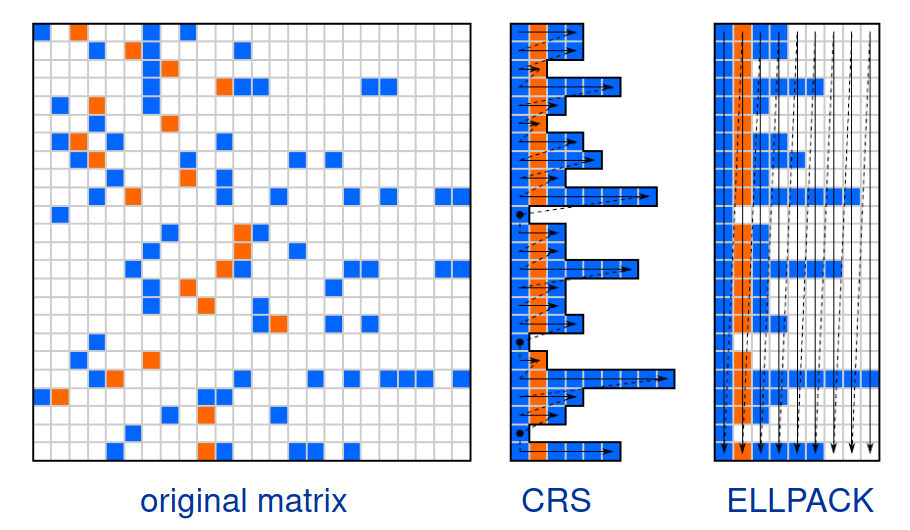
\includegraphics[scale=0.3]{formats.png}  \\
	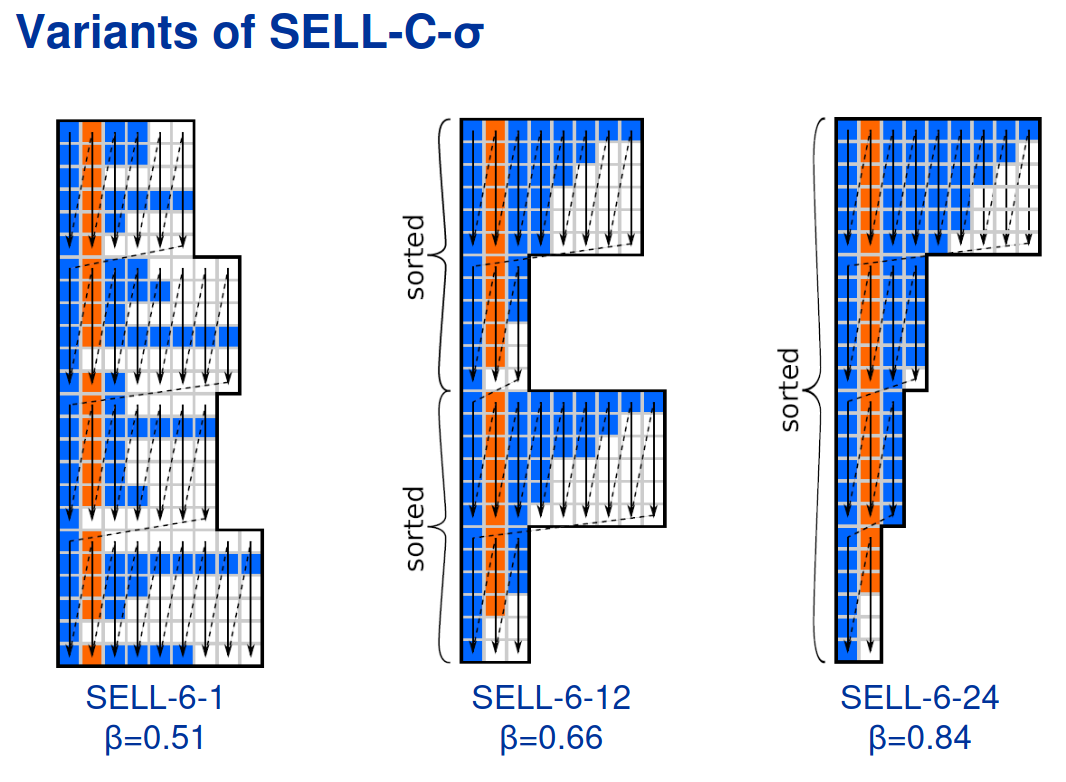
\includegraphics[scale=0.23]{sellc.png}  
	\caption{ Illustration of matrix formats from \ref{formats}.  }
	\label{formats}
\end{figure}





\section{Implementation}

\subsection{CSR}
To implement scalar CSR, we use three arrays as described below.  
 \begin{figure}[h]
	\centering
	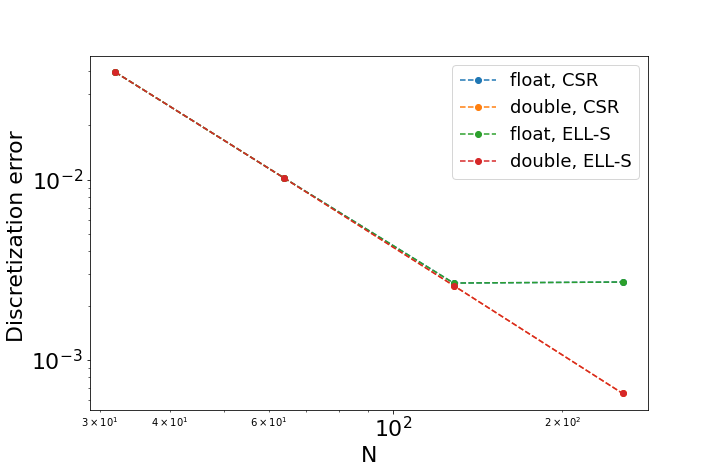
\includegraphics[scale=0.36]{errors.png}  
	\caption{ Discretization errors as a function of N. Just  for checking the correctness of implementation.  }
	\label{erros}
\end{figure}
 
 We measure memory bandwidth and computational performance. As expected, the performance values for runnings on GPU are  higher than for CPU. Figure \ref{perf} illustrates obtained results. Obtained maximum is 452.416 Gb/s which is only half of theoretical value.  The times for copy matrix and vectors to devises are higher $\approx$50 times the computations.   
 \begin{figure}[h]
	\centering
	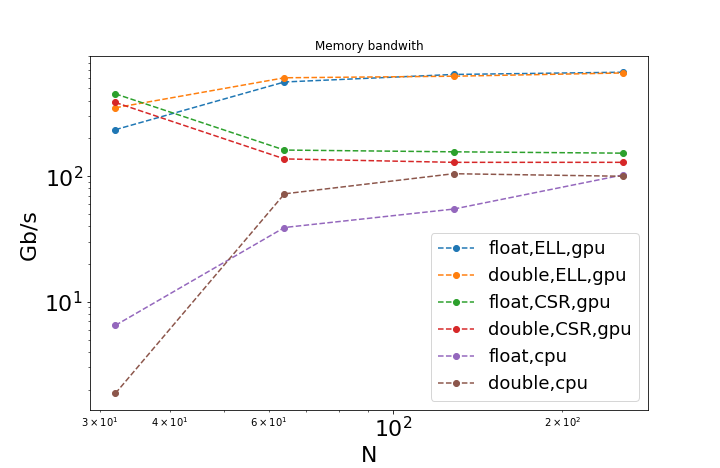
\includegraphics[scale=0.36]{memorybandwidth.png}  \\
	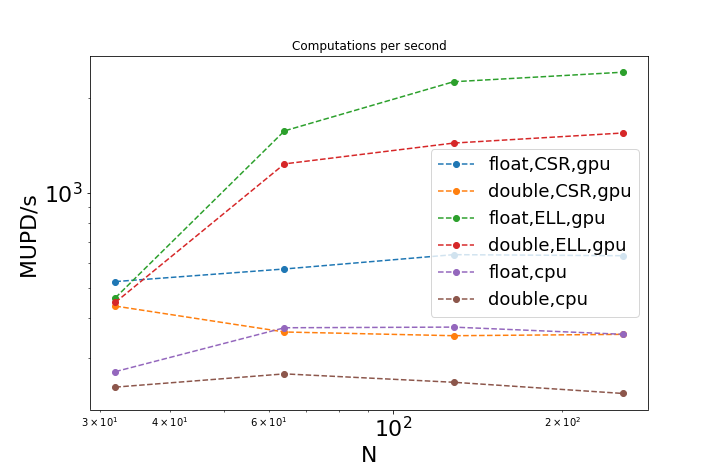
\includegraphics[scale=0.36]{comp.png}  
	\caption{Performance obtained for using CSR format. For CPU, we use 16 processes.  }
	\label{perf}
\end{figure}

 
 
 \newpage
 \begin{thebibliography}{9}
 
\bibitem{sell}
Kreutzer, M., Hager, G., Wellein, G., Fehske, H., Bishop, A. R. (2014). A unified sparse matrix data format for efficient general sparse matrix-vector multiplication on modern processors with wide SIMD units. SIAM Journal on Scientific Computing, 36(5), C401-C423. 


 \end{thebibliography}

%\end{thebibliography}

\end{document}
